\documentclass[twocolumn]{article}

%\usepackage[iso]{umlaute}
%\usepackage{german}
\usepackage{graphicx}
\setlength{\parindent}{0cm}
\setlength{\parskip}{1ex}
\setlength{\columnsep}{25pt}

\textwidth=17cm
\textheight=23cm
\setlength{\unitlength}{0.5cm}
\setlength{\parindent}{0.0cm}
\setlength{\parskip}{1ex}
\raggedbottom
\sloppy
%\addtolength{\evensidemargin}{-5cm}
\addtolength{\oddsidemargin}{-1.5cm}
\addtolength{\topmargin}{-2cm}

\sloppy

% Your name
\author{Trung Nguyen\\ Technische Universit\"at M\"unchen}

\title{Seminar Cloud Computing \\
       {\bf From Concept to Production: Enablements TinyML in Industrial Setting}
}

% Date of your talk
\date{November 2024}

\usepackage{hyperref}

\begin{document}

\maketitle

\begin{abstract}
In recent years, Artificial Intelligence (AI) and Machine Learning (ML) have received tremendous amount of attention in both industry and research world. However, conventional Machine Learning demands high computing capability which limits its usage to only larger computing units. The pardigm shift to Tiny Machine Learning (TinyML) is revolutionizing industries by enabling the deployment of machine learning models on low-power, resource-constrained devices. Being one of the most rapid developing field of Machine Learning, TinyML promises to benifits multiple industries. However, building a production-ready tinyML system poses different unique challenges. In this paper, we explore the key obstacles faced when developing and deploying TinyML models in production environments, including model optimization, hardware limitations, software integration, and maintaining performance in real-world conditions. Additionally, we present real-world use cases of TinyML in industrial settings, showcasing its transformative impact. We also discuss practical approaches and strategies presented by recent researches \cite{ren_tinyol_2021} to overcome these challenges, providing insights into how TinyML systems can be successfully scaled and implemented in production.
\end{abstract}

% \section defines numbered parts of the paper with titles
% there also are \subsection and \subsubsection
\section{Introduction}
\label{introduction}


Traditional Machine Learning Models, especially Deep Learning Models typically require substantial amount of computing capability to operate effectively. These models are often trained on powerful Graphics Processing Units (GPUs) and produce large models ranging from tens or hundreds of gigabytes (GB) down to smaller models in the range of 10 to 100 megabytes (MB). However, the memory requirements during runtime for these models far exceed what microcontrollers (MCUs) can handle.
The pardigm shift to TinyML is driven by the prevailing number of Microcontroller Units (MCU) currently circulating in the industry. According to a recent report \cite{noauthor_microcontroller_nodate,grandviewresearch_research_2023}, as of 2021, around 31 billion MCUs were shipped worldwide annually. The MCU market size is projected to increase in upcoming years \cite{noauthor_microcontroller_nodate}. This creates a big incentive for researchers and industry players to put effort into developing the technology further.
TinyML aims to enable data processing or inferencing directly on embedded systems, particularly on Internet Of Things (IOT), instead of streaming to the cloud. TinyML model can run on energy-, and memory-constraint devices by limiting communication overhead with better suited architecture design and applying different compressing techniques such as: quantization and pruning. The advancement of tinyML has positively influenced multiple industries/sectors such as: industrial IOT \cite{ray_review_2022}, healthcare \cite{bhamare_chapter_2024}, agriculture \cite{tsoukas_tinyml-based_2022}, IOT in smart-city \cite{hussein_original_2024,ray_review_2022}. \\[0.25cm]

Although various organizations have been actively investing resources into machine learning projects, only around 13\% of these projects successfully progress to production. This low success rate highlights the complex challenges and gaps in translating ML concepts into fully functional, production-grade systems, especially in the realm of TinyML. In this paper, we aim to address these challenges and outline what is necessary to transition a TinyML project from concept to production, ultimately creating value for industrial applications. In Chapter~\ref{tinyml_overview}, we provide an in-depth overview of the fundamental concepts, techniques, and development pipeline of TinyML. Following this, in Chapter~\ref{prod_tinyml}, we draw on recent research to investigate the specific challenges encountered in developing and deploying TinyML models in production environments, as well as practical strategies to overcome these obstacles. Next, in Chapter~\ref{use_cases}, we explore real-world applications of TinyML in industrial settings, illustrating its transformative potential. Finally, in Chapter~\ref{future_of_tinyml}, we consider the future trajectory of TinyML, discussing upcoming advancements and their implications for broader industrial adoption.
\begin{figure}
	\centerline{
	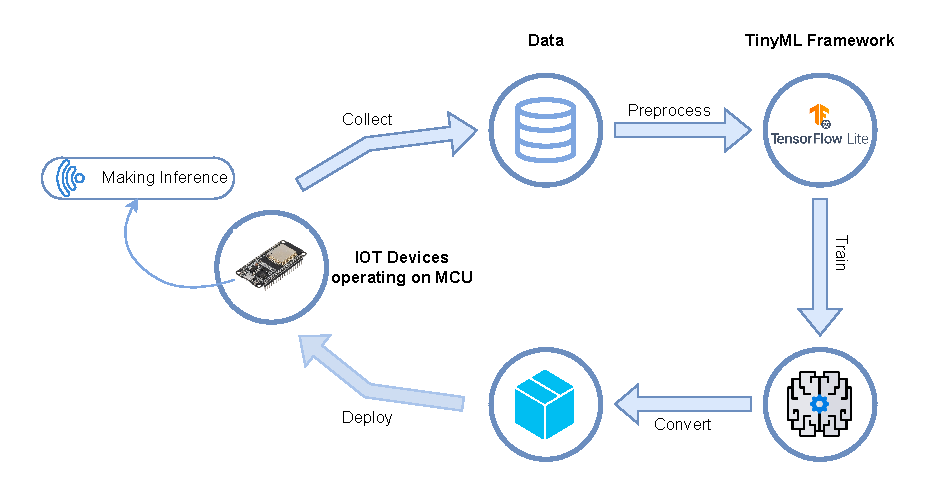
\includegraphics[width=1\columnwidth]{resource/tinyml_deployment.pdf}
	}
	\caption{The caption explaining what can be seen in the image/figure.
	Readers often read captions first if they do not have much time. Thus,
	it is important to find a good short explanation.}
	% A label to allow refering to this figure in the text.
	\label{TUM}
\end{figure}

\section{TinyML Overview} 
\label{tinyml_overview}

\subsection{Key Concepts and Techniques}

Pruning removes unnecessary neurons or connections from a neural network to reduce its size and complexity. This optimization lowers memory and computational demands, making the model faster and more efficient for deployment on resource-limited devices like microcontrollers.

Quantization reduces the precision of model parameters (e.g., from 32-bit to 8-bit), which decreases model size and computational needs. This technique enables efficient model inference on devices with limited memory and processing power, such as those used in TinyML applications.

With the TinyML model running on edge, the data is stored, processed and analysed internally rather
than at an external server or cloud. 

\subsection{TinyML pipeline}

\paragraph{Data Collection:}
	The workflow starts with collecting data from an IoT device. This data serves as the input for training machine learning models. The IoT device can gather various types of data depending on the application, such as sensor data in smart homes or environmental monitoring. \\[0.25cm]
\paragraph{Preprocessing:}
	After collecting data, it moves to the preprocessing stage. Here, the data is cleaned and prepared for model training. Preprocessing can involve tasks such as normalization, handling missing values, or feature extraction to improve the quality of the input data.\\[0.25cm]
\paragraph{Model Training:}
	The preprocessed data is fed into an ML framework, where a machine learning model is trained. This stage involves using machine learning algorithms to find patterns in the data, building a predictive or analytical model that can generalize from the data.\\[0.25cm]
\paragraph{Model Conversion:}
	Once the model is trained, it is converted into a format suitable for deployment on resource-constrained devices, like microcontrollers. This step might involve techniques such as quantization (reducing the precision of model weights) or pruning (removing unnecessary parts of the model) to reduce the model’s size and computation needs.\\[0.25cm]
\paragraph{Model Packaging:}
	After conversion, the model is packaged into a deployable form. This includes bundling the model with any necessary runtime components to allow it to be executed efficiently on the target device.\\[0.25cm]
\paragraph{Deployment:}
	The next step involves deploying the packaged model onto an IoT device. This means transferring the model to the device, setting it up for real-time inference or operation in the field.\\[0.25cm]
\paragraph{Inference:}
	Finally, the deployed model performs inference on the IoT device. Inference refers to the process of using the model to make predictions or decisions based on new data collected by the IoT device. The model operates locally on the device without needing continuous cloud connectivity, enabling real-time decision-making at the edge.\\[0.25cm]



\section{Enablements of TinyML in Industrial Setting}
\label{prod_tinyml}

\subsection{Challenges}

The fundamental pipeline for deploying a TinyML model to a microcontroller, as described above, provides a general framework for model development and deployment. However, in industrial settings, this pipeline often falls short due to a variety of challenges unique to production environments.

\subsubsection{Adaptation to unseen scenarios and constantly changing conditions}
In Traditional ML, operating model can be constantly update via good internet connection. It is however not the case with tinyML model on MCUs. This is due to those IOT devices or edge devices usually don't have constant connection to the internet or to the cloud. It is often the case that once a model is deployed on MCU, It will be in operation for a while.
This vastly affects the deployed tinyML model overtime. // explain: ... 

Real-world conditions are subject to constant change. Static model can struggle to adapt to changing input data patterns, a problem known as con- cept drift and data drift, resulting in performance degradation.

To tackle this, we have found approaches from Paper A, Paper B.

\subsubsection{Performance across heterogeneous devices or affected by heterogeneity}

\paragraph{Hardware} TinyML models are deployed on a diverse range of hardware architectures, including microcontrollers, embedded systems, and IoT devices. These platforms vary significantly in processor type (e.g., ARM or RISC-V), clock speeds, memory capacities, and specialized hardware accelerators. Each hardware platform presents its own set of constraints and requires unique optimizations, making it difficult to design models that perform consistently well across devices. Additionally, a key challenge in deploying TinyML models across different hardware is the lack of standardized metrics for comparing performance, as noted by Banbury et al. (2020). This variation complicates efforts to ensure uniform and predictable results across multiple implementations.

\paragraph{Software} Different microcontrollers (MCUs) are often tied to distinct programming frameworks, each with specific compatibility limitations and restrictions. This diversity in frameworks leads to inconsistencies in model development and deployment, as the availability and compatibility of ML frameworks vary across platforms. Furthermore, the use of different libraries, inference engines, and compilers adds layers of complexity, making it challenging to maintain a streamlined deployment process across different MCUs. These software inconsistencies require careful management to avoid compatibility issues that could hinder TinyML applications on various devices.

\paragraph{Data Heterogeneity} Ensuring model accuracy across devices depends on managing data quality and addressing issues such as noisy or missing data (Kallimani et al., 2023). Variations in data distribution between devices can significantly impact model performance during deployment, requiring models to be robust to a wide range of inputs. Data heterogeneity also affects TinyML application portability (Lakshman \& Eisty, 2022), as models must adapt to different data distributions encountered across devices. This need for adaptability drives the implementation of preprocessing, transfer learning, and generalization techniques, which help maintain consistent performance despite variations in data and device contexts.

To tackle this, we have found approaches from Paper A, Paper B.



\subsubsection{Integrating with Existing IOT System}
Integrating TinyML-enabled microcontrollers (MCUs) into existing IoT systems presents several unique challenges. IoT infrastructures are often built on established architectures, protocols, and data formats that may not be directly compatible with TinyML MCUs. Adapting these MCUs to work within the existing IoT ecosystem requires significant customization to ensure seamless data exchange, communication, and interoperability.

Moreover, existing IoT systems frequently rely on centralized processing or cloud-based analytics, while TinyML emphasizes local computation on edge devices. This architectural shift introduces complexities in synchronizing data and managing hybrid workflows that combine cloud and edge processing. Industrial IoT deployments also come with strict security and compliance requirements, so integrating TinyML MCUs necessitates additional security protocols, device authentication, and data encryption to maintain data integrity across the IoT network.

Maintenance and scalability issues can complicate the integration of TinyML into IoT systems at scale. Updating models on distributed MCUs, managing firmware compatibility, and monitoring device health require robust infrastructure and automated processes, adding layers of complexity to deploying and managing TinyML solutions within existing IoT frameworks.

This urges the need for a sufficient method to manage and maintain TinyML system at scale.

To tackle this, we have found approaches from Paper A, Paper B.

% use \cite to refer to papers from seminarpaper.bib
% this file is processed by bibtex, and it automatically adds numbering
\cite{hussein_original_2024, paul_rethinking_2021, de_prado_robustifying_2020,ren_synergy_2021,roshan_adaptive_2021}.


\subsection{Bringing tinyML to production environment}
\subsubsection{Advanced On Device Learning Methods }
TinyOL (Tiny Machine Learning with Online Learning), as presented in the paper, is a framework designed to enable on-device learning. This means it allows models deployed on embedded devices (like sensors or microcontrollers) to learn and adapt in real-time without needing to be retrained externally. Here’s how it works and why it doesn’t require an internet 
\paragraph{On-device Incremental Learning} TinyOL enables continuous learning directly on resource-constrained devices. It can train a model incrementally by learning from streaming data as it arrives in real-time, without the need to store large datasets. This approach allows the model to remain updated with new data without requiring frequent retraining in centralized, powerful systems.
\paragraph{Adapt} TinyOL is particularly useful in cases where the environment is dynamic and subject to changes. As new data arrives, the model adjusts incrementally, making it more robust to “concept drift” (changes in data patterns over time) without requiring access to previous data. This is critical in real-world scenarios where conditions may fluctuate frequently. 
\paragraph{Minimal Resource consumption}TinyOL operates with minimal memory and computational resources. For instance, the framework can run within just 7 KB of RAM and 135 KB of Flash memory, making it suitable for low-power embedded devices that cannot support traditional machine learning models.

\paragraph{How TinyOL Works}

\begin{enumerate}
    \item The device collects streaming data from its environment.
    \item TinyOL processes the data, updates the model’s running mean and variance, and adjusts the model weights accordingly.
    \item After processing each new data point, the model discards the data, ensuring efficient memory usage.
    \item The model is continuously updated, allowing it to handle shifts in data patterns over time.
\end{enumerate}
\subsubsection{Meta-Learning Framework and semantic management tools }

TinyML models often need to be deployed on a wide range of embedded devices that differ in terms of hardware, environmental conditions, and tasks. A key challenge is how to ensure that these models perform well across different devices, even when they face different data distributions, goals, and constraints. Training a universal model for all devices is impractical because of limited labeled data and diverse deployment environments. This is where TinyReptile and TinyMetaFed come in.

SeLoC-ML addresses the challenges of managing a fragmented TinyML ecosystem where numerous TinyML models need to be deployed on different embedded devices, each with unique hardware, sensors, and computational limits. Traditional TinyML deployment requires significant technical expertise, but SeLoC-ML simplifies this by:

	1.	Streamlining Model and Device Matching: Using a centralized knowledge graph to manage both TinyML models and embedded devices, ensuring quick discovery and compatibility matching.
	2.	Automating Deployment: By providing an easy-to-use low-code interface, it helps non-experts deploy TinyML models without needing deep technical knowledge.

\subsubsection{Low-code management system}


MLOps for Scaling TinyML: TinyMLOps has some drawbacks

The paper introduces a TinyML low-code management system called SeLoC-ML, designed to simplify the deployment, management, and scaling of TinyML applications. This system is built on semantic web technology and integrates with Mendix, a low-code platform, to enable non-experts to manage and deploy TinyML models across diverse embedded devices.

Workflow of SeLoC-ML

\begin{enumerate}
	\item Define Requirements: Users specify the model requirements or device specifications (e.g., sensor types, memory limits) via the Mendix interface.
	\item	Match Models and Devices: The system queries the KG for matching models and devices based on the user’s input. The system ensures that the selected models meet the hardware constraints of the device.
	\item	Generate Deployment Code: Once a model and device are matched, SeLoC-ML generates a deployment project, including configuration files and scripts, which are ready to be uploaded to the target hardware. This eliminates the need for manual coding, reducing development time and errors.
	\item	Deploy and Manage at Scale: SeLoC-ML supports large-scale management, allowing users to track, update, and maintain TinyML models across multiple devices.
\end{enumerate}


\section{Use Cases of TinyML in Industrial Setting}
\label{use_cases}

Enumerations using bullet points:

\begin{itemize}
	\item 	Agriculture
	\item 	Environmental Monitoring
	\item 	Industrial predictive maintenance
	\item 	Edge AI and Autonomous Systems
\end{itemize}


\section{Future of TinyML }
\label{future_of_tinyml}



\section{Conclusion}
\label{conclusion}



% Put citations from bibtex into References section which were not
% explicity cited.
\nocite{hussein_original_2024,paul_rethinking_2021}


\bibliographystyle{plain}
% Literature sources are to be found in seminarpaper.bib
\bibliography{seminarpaper}
\end{document}
